

\chapter{INTRODUCTION}
\label{chap:Introduction}
% Change to arabic page numbers at chapter 1
\pagenumbering{arabic}

\section{NASA Magnetospheric MultiScale Mission}
\label{sec:NASAMagnetosphericMultiScaleMission}

NASA's Magnetospheric MultiScale (MMS) Mission is a Solar Terrestrial probe mission scheduled for launch in March 2015 \cite{mms_website}.  The mission consists of four identical satellites orbiting the Earth in a constellation formation flight.  Construction of the satellites is occurring at NASA's Goddard Space Flight Center (GSFC) where they are being equipped to study the microphysics of magnetic reconnection events within the Earth's magnetic fields.

\begin{figure}[H]
  \centerline{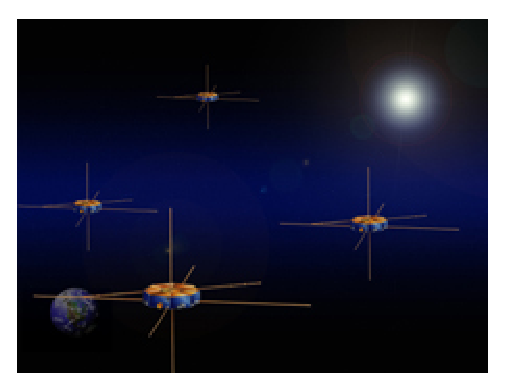
\psfig{file=figures/mms_spacecraft_formation.eps,height=2.4in}}
  \caption{MMS Spacecraft Formation \cite{mms_website}}
  \label{fig:spacecraft_formation}
\end{figure}

A reconnection event occurs when magnetic field lines cross allowing energetic particles to traverse from interstellar space into the Earth's magnetosphere releasing large quantities of heat and kinetic energy.  The diffusion region of a reconnection event starts on the day side magnetopause and quickly folds over to the Earth's magnetotail (Figure \ref{fig:magneticfields}).  This region is only 1-10 km in size but can travel at 10-100 km/hr \cite{swri} making it extremely difficult to measure.  Effects of a reconnection event are regularly experienced via the aurora borealis, interference with spacecraft GPS systems, and disruptions to electrical grids and communication networks.

\begin{figure}[H]
  \centerline{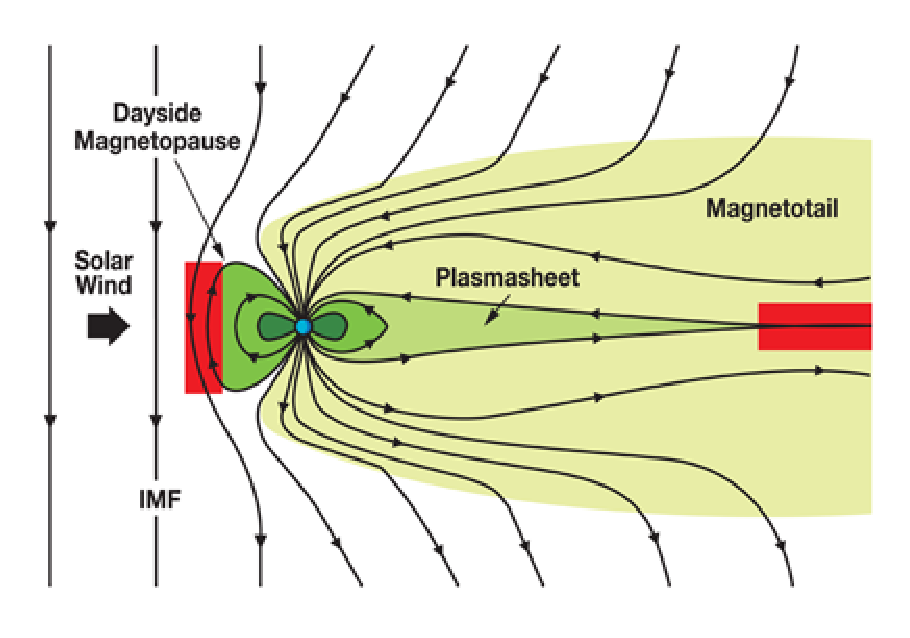
\psfig{file=figures/2d_earth_mag_field_lines.eps,height=3in}}
  \caption{Cross section of Earth's magnetic field \cite{mms_website}}
  \label{fig:magneticfields}
\end{figure}

Despite the widely experienced effects of reconnection events, very little about the microphysics inside its the diffusion region has been adequately quantified.  Magnetometers, spectrometers, and other equipment currently in orbit are only able to capture a small fraction of the event's behavior.  Most equipment collect data from a single point or direction in space or some can get a $360^o$ view of space by applying a slow spin to the spacecraft.  Both of these measurement methods are insufficient at capturing the structure of the diffusion region as it passes.

MMS's four satellites are equipped with instrumentation mounted at the end of six boom extending out from the spacecraft's body along each major axis.  Four Spin Plane Double Probes (SDP) booms and two Axial Double Probes (ADP) booms.  This configuration along with high resolution electron and ion spectrometers gives the constellation a new insight into the internal structure of the diffusion region.

Placing the instrumentation at the ends of the booms is an advantage to the science portion of the mission but creates a unique challenge for the Attitude Determination and Control Systems (ADCS).  The satellites are spin-stabilized at a rate of 3 rpm, and disturbances to the rotation could translate into undesirable boom dynamics and body nutation.

\begin{figure}[H]
  \centerline{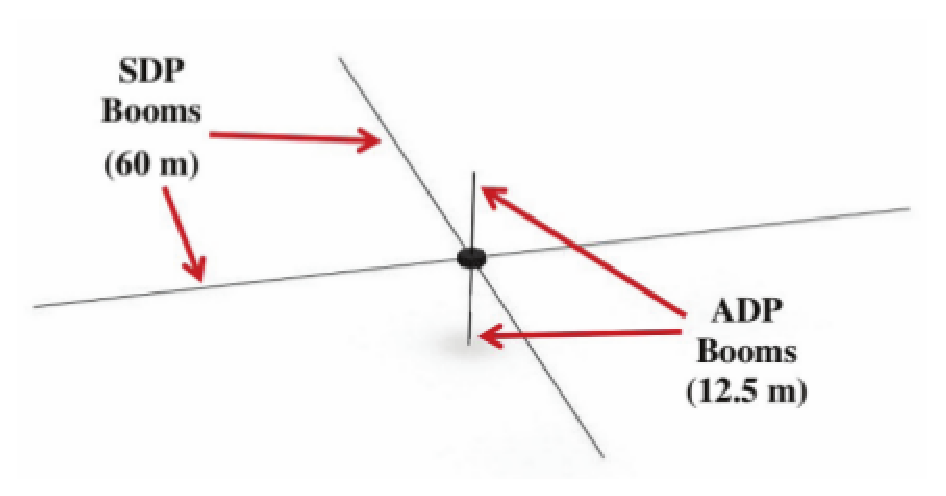
\psfig{file=figures/booms.eps,height=2in}}
  \caption{MMS Boom Configuration \cite{mushawehthesis}}
  \label{fig:booms}
\end{figure}

Figure \ref{fig:booms}, created by Neil Mushaweh \cite{mushawehthesis}, shows a scale model of one of the MMS satellites.  Mushaweh performed finite element analysis of the boom dynamics and simulation based comparisons of nonlinear observer-based controllers.  His research unveiled a major shortcoming in the current numerical simulation software needed for analyzing the dynamics of a NASA MMS satellite's rotating body with flexible booms.

\begin{quote}{``While attempting to rotate the satellite model at 3 rotations per minute about [the $z$-axis], the inability of the software to transform coordinates after 90 degrees of rotation caused the rotation to cease. When such constraints on coordinate transformations are removed, or when the coordinate system is changed to cylindrical coordinates, the model began to expand in the radial direction. These inaccurate simulation results indicate that there are numerical instabilities that occur in dynamic transient simulations in which rotational motion is experienced. This numerical instability was confirmed by MSC support engineers, and proven to be insurmountable in the scope of this research. Overcoming this numerical instability in dynamic transient analysis through future research could have implications on several design and analysis situations in which coordinate transformations can cause inaccurate results.''~\cite{mushawehthesis}}\end{quote}


% Science questions to answer \cite{mms_website}
%     What determines when reconnection starts and how fast it proceeds?
%     What is the structure of the diffusion region?
%     How do the plasmas and magnetic fields disconnect and reconnect in the diffusion regions?
%     What role do the electrons play in facilitating reconnection?
%     What is the role of turbulence in the reconnection process?
%     How does reconnection lead to the acceleration of particles to high energies?f


% \todo{image of formation flight}
% study microphysics of
%   magnetic reconnection
%   energetic particle acceleration
%   turbulence

% s/c MMS-1, MMS-2..MMS-4
% reconnection: Electromagnetic energy from the sun interacts with Earth's magnetosphere causing magnetic field lines to cross and create a burst of energy \cite{nasa_edge_video_ne_at_mms}
% magnetic reconnection measured ions and electrons as boundary passes to create 3d model of it passing by
% Fast plasma investigation
% probing the electron diffusion region (EDR) (passes too rapidly to get an accurate view with current equipment small (1-10 km) and rapidly moving (10-100 km/s))
% adjacent magnetic fields generally have significantly different orientations such that when they intersect, a large amount of energy is dispursed within a small region in the form of heat and kinetic energy.  The region = diffusion region
% explore magnetic reconnection
% dynamic regions of magnetosphere
% orbits planned to pass through the upstream and downstream magnetic reconnection sites
% 1) day side - solar wind field lines connection
% 2) down stream -
% 3) plasma travels down and causes the Arura
% through magnetospheric reconnection, portals allow energetic particles to traverse from outside to the interior of the magnetosphere
% predict when solar space weather within the magnetosphere and if they will affect orbiting satellites
% adverse space weather within the magnetosphere can negatively impact spacecraft system health GPS, induce disruptive current in electrical grids, communications, increased radiation exposure on trans-polar flights

% Difficult to understand
% magnetic boundary passes satellites quickly so has been hard to measure
% MMS has instruments to capture measurements
% Instruments mounted on all sides of the
% 8 sensors 1/30th sec instead of

% October 2014, Atlas five launch \cite{nasa_edge_video}

% Sensors
%   star sensor -> attitude
%   accelerometers -> $\Delta V$


% Fast Plasma Instrument (FPI) - controls
%   16 Dual Electron spectrometer (DES) Goddard built
%   16 Dual Ion Spectrometer (DIS) Japan *** built, hand delivered
%   180 degree and +- 22 degree measurement
%   30 millisec measurement rate 100x faster than previous missions entire view of sky
% FPI
%   despins data

% Instument Data processing Unit (IDPU) - brains of measurements
%   collects, compresses, transmits requested measurement data
%   configure while on mission

% booms
%   eight deployable booms
%   two 12.5m axial booms (electric field sensors)
%   four 60m wire booms
%   two 5m booms in spin plane for magnetometers
% rigid, wire, top/bottom booms
% important to keep consistent spin rate to get accurate estimates of boom location


% \section{Propulsion}

% types: solid propellents, bi propellents, electro propulsion, cold gas systems
% chose: mono-propellant blowdown - hydrozene power thrusters \cite{nasa_edge_video_propulsion}
% 3 rpm
% radial thrusters - spinning
% axial thrusters - prevent nutation

% concern:
% propulsion introduce distrubances

% 20 second pulses

% fuel limits by number of adjustments


% \section{performance requirements}

% $\pm 0.5$ deg attitude tollerance
% 1/10th of a second

\section{Research Objective}
\label{sec:ResearchObjective}

This thesis utilizes an experimental table top satellite prototype (NASA MMS TableSat 1A) to span two main efforts.  The first is to create a physical model of a satellite for NASA's Magnetospheric MultiScale (MMS) Mission in order to validate and compare varied gyroless attitude determination and control systems (ADCS) techniques.  The ADCS maintains the TableSat constant 3 rpm rotation, prevents boom oscillations, and detects and corrects for unwanted nutation.  The second effort is a software system that can be used to implement theoretical and experimental models.  The system provides near ``real-time'' feedback of the system's states, and allows for ``on-the-fly'' modification to control parameters.  The system is specifically designed such that any control systems engineer is able to customize and extend its functionality without substantial programming expertise.

\section{Past Work}
\label{sec:PastWork}

This work is a direct extension off of Vess' research \cite{vessthesis} of using TableSat through a Numerical Simulation Software (NSS like Matlab Simulink or Octave) and onboard flight controllers to demonstrate fundamentals of control theory.  The TableSat experimental design is modified to study the system dynamics of the instrument booms and nutation actuators in NASA's MMS mission satellites.  Previous experimental \cite{tsat1b} \cite{tsat1c} \cite{tsat2} and analytical \cite{mushawehthesis} ADCS work at University of New Hampshire's Advanced Control Lab (ACL) has been performed targeting the NASA MMS mission.  The TableSat platform or similar derivations have also been adapted in investigate other areas of research including embedded systems development \cite{tablesat_xuml} and fault tolerant control \cite{tablesat_object_bench} \cite{nanjing_university}.


\section{Analytical and Experimental Test Bed}
\label{sec:AnalyticalandExperimentalTestbed}

The test bed used for analytical simulations and experimental validation consists of a base station (laptop) which handles the observer-based controller along with any conversions to and from TableSat sensor and fan voltages, and NASA MMS TableSat 1A which is a wireless limited 3-DOF rotation (full spin and limited nutation) test bed.  Concurrent work has been accomplished in tandem with this research to make improvements to the capabilities of the TableSat system including UNH TableSat 1C \cite{tsat1c} which improves actuator design and reduces rotational friction, and UNH TableSat 2 \cite{tsat2} which adds translation in a plane.

\section{Thesis Contributions}
\label{sec:ThesisContributions}

The research from Vess and Mushaweh illustrate the need for an observer-based controller software system that could be used to perform analytical simulations with spin-stabilized satellites as well as control of their experimental counterpart all while maintaining a high degree of numerical stability.

\subsection{Numerical Stability for Rotational Motion}
\label{subsec:NumericalStabilityforRotationalMotion}

Mushaweh's research using MSC Marc Mentat 2005 r3 and MATLAB / \textit{Simulink}\textsuperscript{TM} R2006a concluded that they were insufficient for simulating the dynamics that exist in a rotating system such as the NASA MMS satellite.  This research contributes and/or incorporates the following attributes into its software to address this deficiency.

\begin{itemize}
  \item \textbf{Quaternion Multiplicative Corrections}: Ensures numerical stability in rotating systems
  \item \textbf{Adaptive Step Algorithms}: Corrects for inconsistent step sizes in simulations or experiments
  \item \textbf{Quaternion Decomposition}: Decouples rotation and nutation control
  \item \textbf{Theta Multiplier with Quaternion Vector Balancing}: Linearly scales quaternion attitude measures used in state corrections without breaking the unit quaternion restriction
  \item \textbf{Euler Axis Based Moments}: Utilizes the quaternion's Euler axis and angular displacement to calculate linearly scaled control moments
\end{itemize}

\subsection{Reusable Software}
\label{subsec:ReusableSoftware}

Since this is an active field of research, future research teams will benefit from the ability to reuse the software created for this thesis in a wide variety of analytical simulations and experimental testing on rotating systems.  In order to make this software an attractive alternative to traditional Numerical Simulation Software, the following principles were incorporated into its design.

\begin{itemize}
  \item \textbf{Concurrent Estimation/Control Algorithms}: Evaluation of multiple estimation and control methods
  \item \textbf{``Run-time'' interface}: Access and visualize the internal state of the control system while running
  \item \textbf{Variable System Clock}: Alter the speed of simulations to compress long simulations or inspect state changes is slow motion
  \item \textbf{Python}: Written in a widely used and expressive language that is easy to learn, comes with ``batteries-included'', and is viable for high performance applications.
  \item \textbf{Modular Design}: Additional estimation or control algorithms or system models can be written and plugged into the existing system
  \item \textbf{Source Agnostic Control System}: Observer-based controller logic can be reused to control a variety of rotating system (simulated and physical)
  \item \textbf{MIT License}: Software will be released publicly on acceptance of this thesis under a MIT License
\end{itemize}

\section{Thesis Outline}
\label{sec:ThesisOutline}

The following chapters are organized as follows:

\begin{itemize}
\item Chapter \ref{chap:SatelliteAttitudeDynamicsAndKinematics}, \nameref{chap:SatelliteAttitudeDynamicsAndKinematics} - This chapter covers the quaternions and body-fixed angular velocities (body rates) parametrization chosen for the state representation of the spin-stabilized satellite, and the dynamics and kinematics involved in modeling it's motion.
\item Chapter \ref{chap:UNHTableSat1A}, \nameref{chap:UNHTableSat1A} - This chapter is a walk through of the components in the UNH NASA MMS TableSat 1A including the how raw sensor voltages are transmitted to the base station for conversion by the controller into a state representation.
\item Chapter \ref{chap:TableSatAttitudeDynamicsSoftware}, \nameref{chap:TableSatAttitudeDynamicsSoftware} - Chapters \ref{chap:SatelliteAttitudeDynamicsAndKinematics} and \ref{chap:UNHTableSat1A} establish the analytical and experimental state representations.  This chapter covers how the state representations with their associated equations of motion are implemented in this thesis' software.
\item Chapter \ref{chap:StateError}, \nameref{chap:StateError} - This chapter details issues with current implementations of quaternion error calculations and covers the development and implementation of the ``Theta Multiplier with Quaternion Vector Balancing'' method for high integrity attitude adjustments.
\item Chapter \ref{chap:Estimators}, \nameref{chap:Estimators} - This chapter focuses on the implementation and performance comparisons of the PID and Sliding Mode Observer (SMO) estimation methods using the chosen state parameterization along with the theta multiplier error correction technique established in Chapter \ref{chap:StateError}.
\item Chapter \ref{chap:Controllers}, \nameref{chap:Controllers} - Similar to Chapter \ref{chap:Estimators}, this chapter compares the performance of PID control and Sliding Mode Control (SMC) methods.  These also include the incorporation of the theta multiplier quaternion error correction method as well as the development and implementation of the ``Euler axis Based Moment'' calculations.
\item Chapter \ref{chap:ObserverBasedControls}, \nameref{chap:ObserverBasedControls} - Performs a comparative analysis of various observer-based controller configurations complete from the input of sensor voltage measurements through voltage to state conversions, state estimation, state control, moment calculation, and calculated actuator voltage settings.
\item Chapter \ref{chap:ProgressionOfControlSystemSoftware}, \nameref{chap:ProgressionOfControlSystemSoftware} - There were four major iterations prior to the final TSatPy solution.  This chapter will cover the advantages and disadvantages to each version as they build to the final solution discussed in Chapter \ref{chap:TSatPy}.
\item Chapter \ref{chap:TSatPy}, \nameref{chap:TSatPy} - This chapter goes into greater depth on the TSatPy software system developed for this thesis including summaries of the main characteristics and modular design.
\item Chapter \ref{chap:Conclusions}, \nameref{chap:Conclusions} - This chapter will summarize the work performed toward the goals of the thesis.
\item Chapter \ref{chap:FutureWork}, \nameref{chap:FutureWork} - This thesis provides a foundation for a system that could be incorporated into a variety of rotational system observer based control systems.  This chapter will detail out areas that could be investigated next.
\item Appendix \ref{chap:tsatpy_samples}, \nameref{chap:tsatpy_samples} - This appendix contains almost all the python scripts used in this thesis for reference.
\item Appendix \ref{chap:tsatpy_source}, \nameref{chap:tsatpy_source} - This is a copy of the source code for the TSatPy software at the time of this publication.  The code will be released under an MIT license at https://github.com/MathYourLife/TSatPy.
\end{itemize}
